\documentclass[margin=10pt]{standalone}
\usepackage{tikz}
\usetikzlibrary{intersections,backgrounds}
\begin{document}

% List of colors
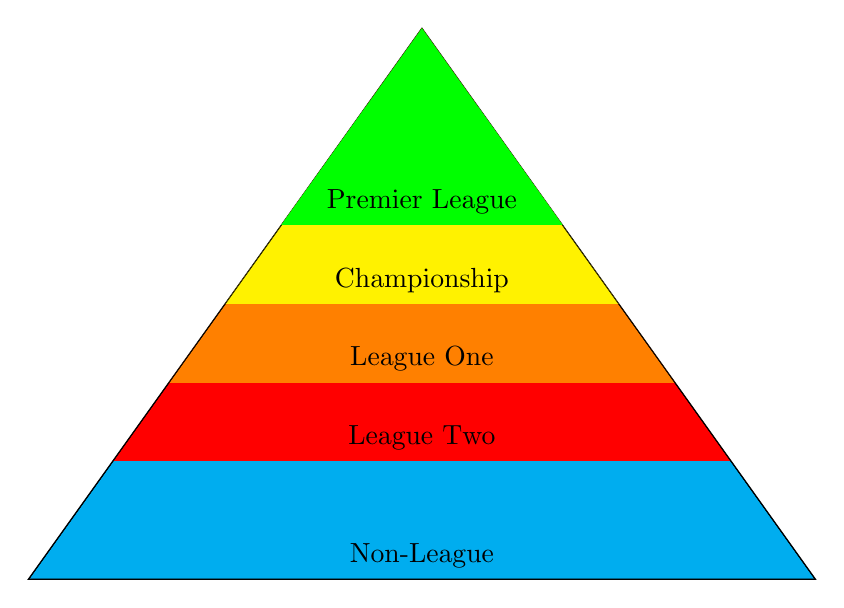
\begin{tikzpicture}
\def\colorlist{{"cyan", "red", "orange", "yellow", "green", "gray", "blue", "violet"}}

\foreach \y/\A [count=\xi starting from 0, evaluate=\y as \nexty using (\y+1.5, evaluate=\xi as \grad using int(\xi*15)] in {0/Non-League, 1.5/League Two,2.5/ League One,3.5/Championship,4.5/Premier League} {%
    \pgfmathsetmacro\myfill{\colorlist[\xi]}
    \begin{scope}[on background layer]
    \clip[preaction={draw}] (-5,0) -- (5,0) -- (0,7) -- cycle;
    \fill[\myfill] (-5,\y) rectangle (5,\nexty);
    \fill[\myfill] (-5,4.5) rectangle (5,7);
    \end{scope}
    \node at (0,\y+.3) {\A};
}
\end{tikzpicture}

% Gradations
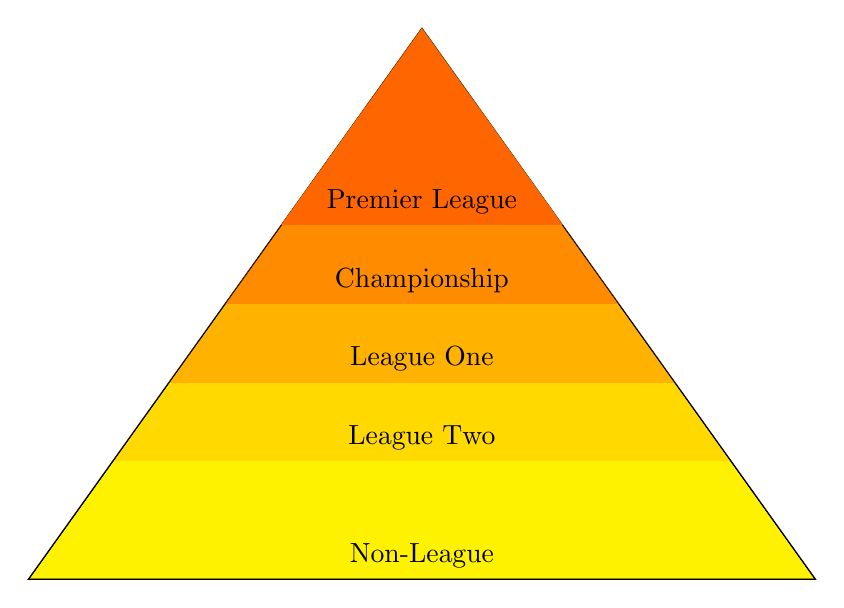
\begin{tikzpicture}[xshift=5cm]
\foreach \y/\A [count=\xi starting from 0, evaluate=\y as \nexty using (\y+1.5, evaluate=\xi as \grad using int(\xi*15)] in {0/Non-League, 1.5/League Two,2.5/ League One,3.5/Championship,4.5/Premier League} {%
    \begin{scope}[on background layer]
    \clip[preaction={draw}] (-5,0) -- (5,0) -- (0,7) -- cycle;
    \fill[red!\grad!yellow] (-5,\y) rectangle (5,\nexty);
    \fill[red!\grad!yellow] (-5,4.5) rectangle (5,7);
    \end{scope}
    \node at (0,\y+.3) {\A};
}
\end{tikzpicture}
\end{document}
